% Please add the following required packages to your document preamble:
% \usepackage{multirow}
\begin{table}[]
\centering
\begin{tabularx}{\textwidth}{lllllll}
\cline{1-4}
\multicolumn{2}{|l|}{\multirow{2}{*}{}}                                  & \multicolumn{2}{c|}{values}                                        &  &  &  \\ \cline{3-4}
\multicolumn{2}{|l|}{}                                                   & \multicolumn{1}{l|}{categorical} & \multicolumn{1}{l|}{quantitative} &  &  &  \\ \cline{1-4}
\multicolumn{1}{|l|}{\multirow{2}{*}{keys}} & \multicolumn{1}{l|}{categorical}   & \multicolumn{1}{l|}{\includegraphics[height=.15\textheight]{figs/catcat.png}}           & \multicolumn{1}{l|}{\includegraphics[height=.15\textheight]{figs/quantcat.png}}          &  &  &  \\ \cline{2-4}
\multicolumn{1}{|l|}{}                      & \multicolumn{1}{l|}{quantitative} & \multicolumn{1}{l|}{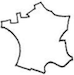
\includegraphics[height=.15\textheight]{figs/catquant.png}}           & \multicolumn{1}{l|}{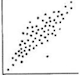
\includegraphics[height=.15\textheight]{figs/quantquant.png}}          &  &  &  \\ \cline{1-4}
                                            &                            &                                  &                                 &  &  &  \\
                                            &                            &                                  &                                 &  &  &  \\
                                            &                            &                                  &                                 &  &  & 
\end{tabularx}
\caption{Bertin's Visualizations of Observations}

\end{table}